% Gemini theme
% See: https://rev.cs.uchicago.edu/k4rtik/gemini-uccs
% A fork of https://github.com/anishathalye/gemini

\documentclass[final]{beamer}

% ====================
% Packages
% ====================

\usepackage[T1]{fontenc}
\usepackage{lmodern}
\usepackage[size=custom,width=121.92,height=60.96,scale=1.0]{beamerposter}
\usetheme{gemini}
% \usecolortheme{uchicago}
\usecolortheme{stanford}
\usepackage{graphicx}
\usepackage{booktabs}
\usepackage{tikz}
\usepackage{pgfplots}
\usepackage[most]{tcolorbox}
\usepackage[export]{adjustbox}
\pgfplotsset{compat=1.17}

\definecolor{mycolor}{RGB}{173,10,29}

\AtBeginDocument{
  \fontsize{32pt}{0.5ex} % Adjust 12pt to your desired font size, and 14pt to a suitable line spacing
}

% ====================
% Lengths
% ====================

% If you have N columns, choose \sepwidth and \colwidth such that
% (N+1)*\sepwidth + N*\colwidth = \paperwidth
\newlength{\sepwidth}
\newlength{\colwidth}
\newlength{\widecolwidth}
\setlength{\sepwidth}{0.0001\paperwidth}
\setlength{\colwidth}{45cm}
\setlength{\widecolwidth}{60cm}

\title{From Possible to Pause-able:\linebreak Children's hesitancy may mark implicit skepticism of incorrect intuitive beliefs}

\author{Adani B. Abutto\inst{a, b, d} \and Igor Bascandziev\inst{a} \and Caren Walker\inst{c} \and Elizabeth Bonawitz\inst{a}}

\institute[shortinst]{\inst{a} Harvard Graduate School of Education \samelineand \inst{b} Stanford University \samelineand \inst{c} University of California San Diego \samelineand \inst{d} LMU Munich}

% ====================
% Footer (optional)
% ====================

\footercontent{
  \hspace{10ex}We thank families for their participation, and the Caplan Foundation, James S. McDonnell Foundation, and Jacobs Foundation for their generous support of this research. \hfill
  Contact: \href{mailto:aabutto@stanford.edu}{aabutto@stanford.edu}  || \href{https://adaniabutto.com}{stanford.edu/$\sim$aabutto}\hspace{10ex}}

% ====================
% Logo (optional)
% ====================

% use this to include logos on the left and/or right side of the header:
 \logoright{
\includegraphics[height=7.5cm]{stanford_logos/hgse_logo_clear.png}}
 \logoleft{
\includegraphics[height=7.5cm]{stanford_logos/CoCoDev_Logo.png}}

% ====================
% Body
% ====================

\begin{document}

\begin{frame}[t]
\begin{columns}[t]

\begin{column}{\colwidth}

  \begin{block}{BACKGROUND}

    \begin{itemize}
      \item Young \textbf{children’s naive, intuitive beliefs} about the material world (e.g., “air is nothing," “a grain of rice weighs nothing”) are theory-like but \textbf{run counter to scientific understanding} \textsuperscript{[1, 2]}
      \item  \textbf{Even \emph{before} acquiring beliefs aligned with scientific understanding}, learners’ \textbf{naive beliefs may conflict} with other parts of their knowledge (e.g., “air is nothing"; "we need air to breathe”)
       \item Elementary schoolers wrestling with such conflicting beliefs may respond more slowly to "incongruent" questions even \emph{before} learning the scientifically correct response
    \end{itemize}
    
	\begin{tcolorbox}[
		colback=mycolor,
		colframe=mycolor,
		coltext=white,
		boxsep=4pt,
		left=2mm,
		right=2mm,
		top=2mm,
		bottom=2mm,
		arc=5mm,
		auto outer arc,
		boxrule=4pt,
		width=\dimexpr\linewidth-2\fboxsep\relax,
		]
		\centering
		\textbf{Among children with naive beliefs about the material world, are response times (RTs) slower for ”theory-incongruent” questions than for ”theory-congruent” questions?}
	\end{tcolorbox}


  \end{block}

  \begin{block}{PROCEDURE}
  
  Children answered 30 forced-choice questions about 10 entities and their physical properties.
    
    \begin{figure}
      \centering
	{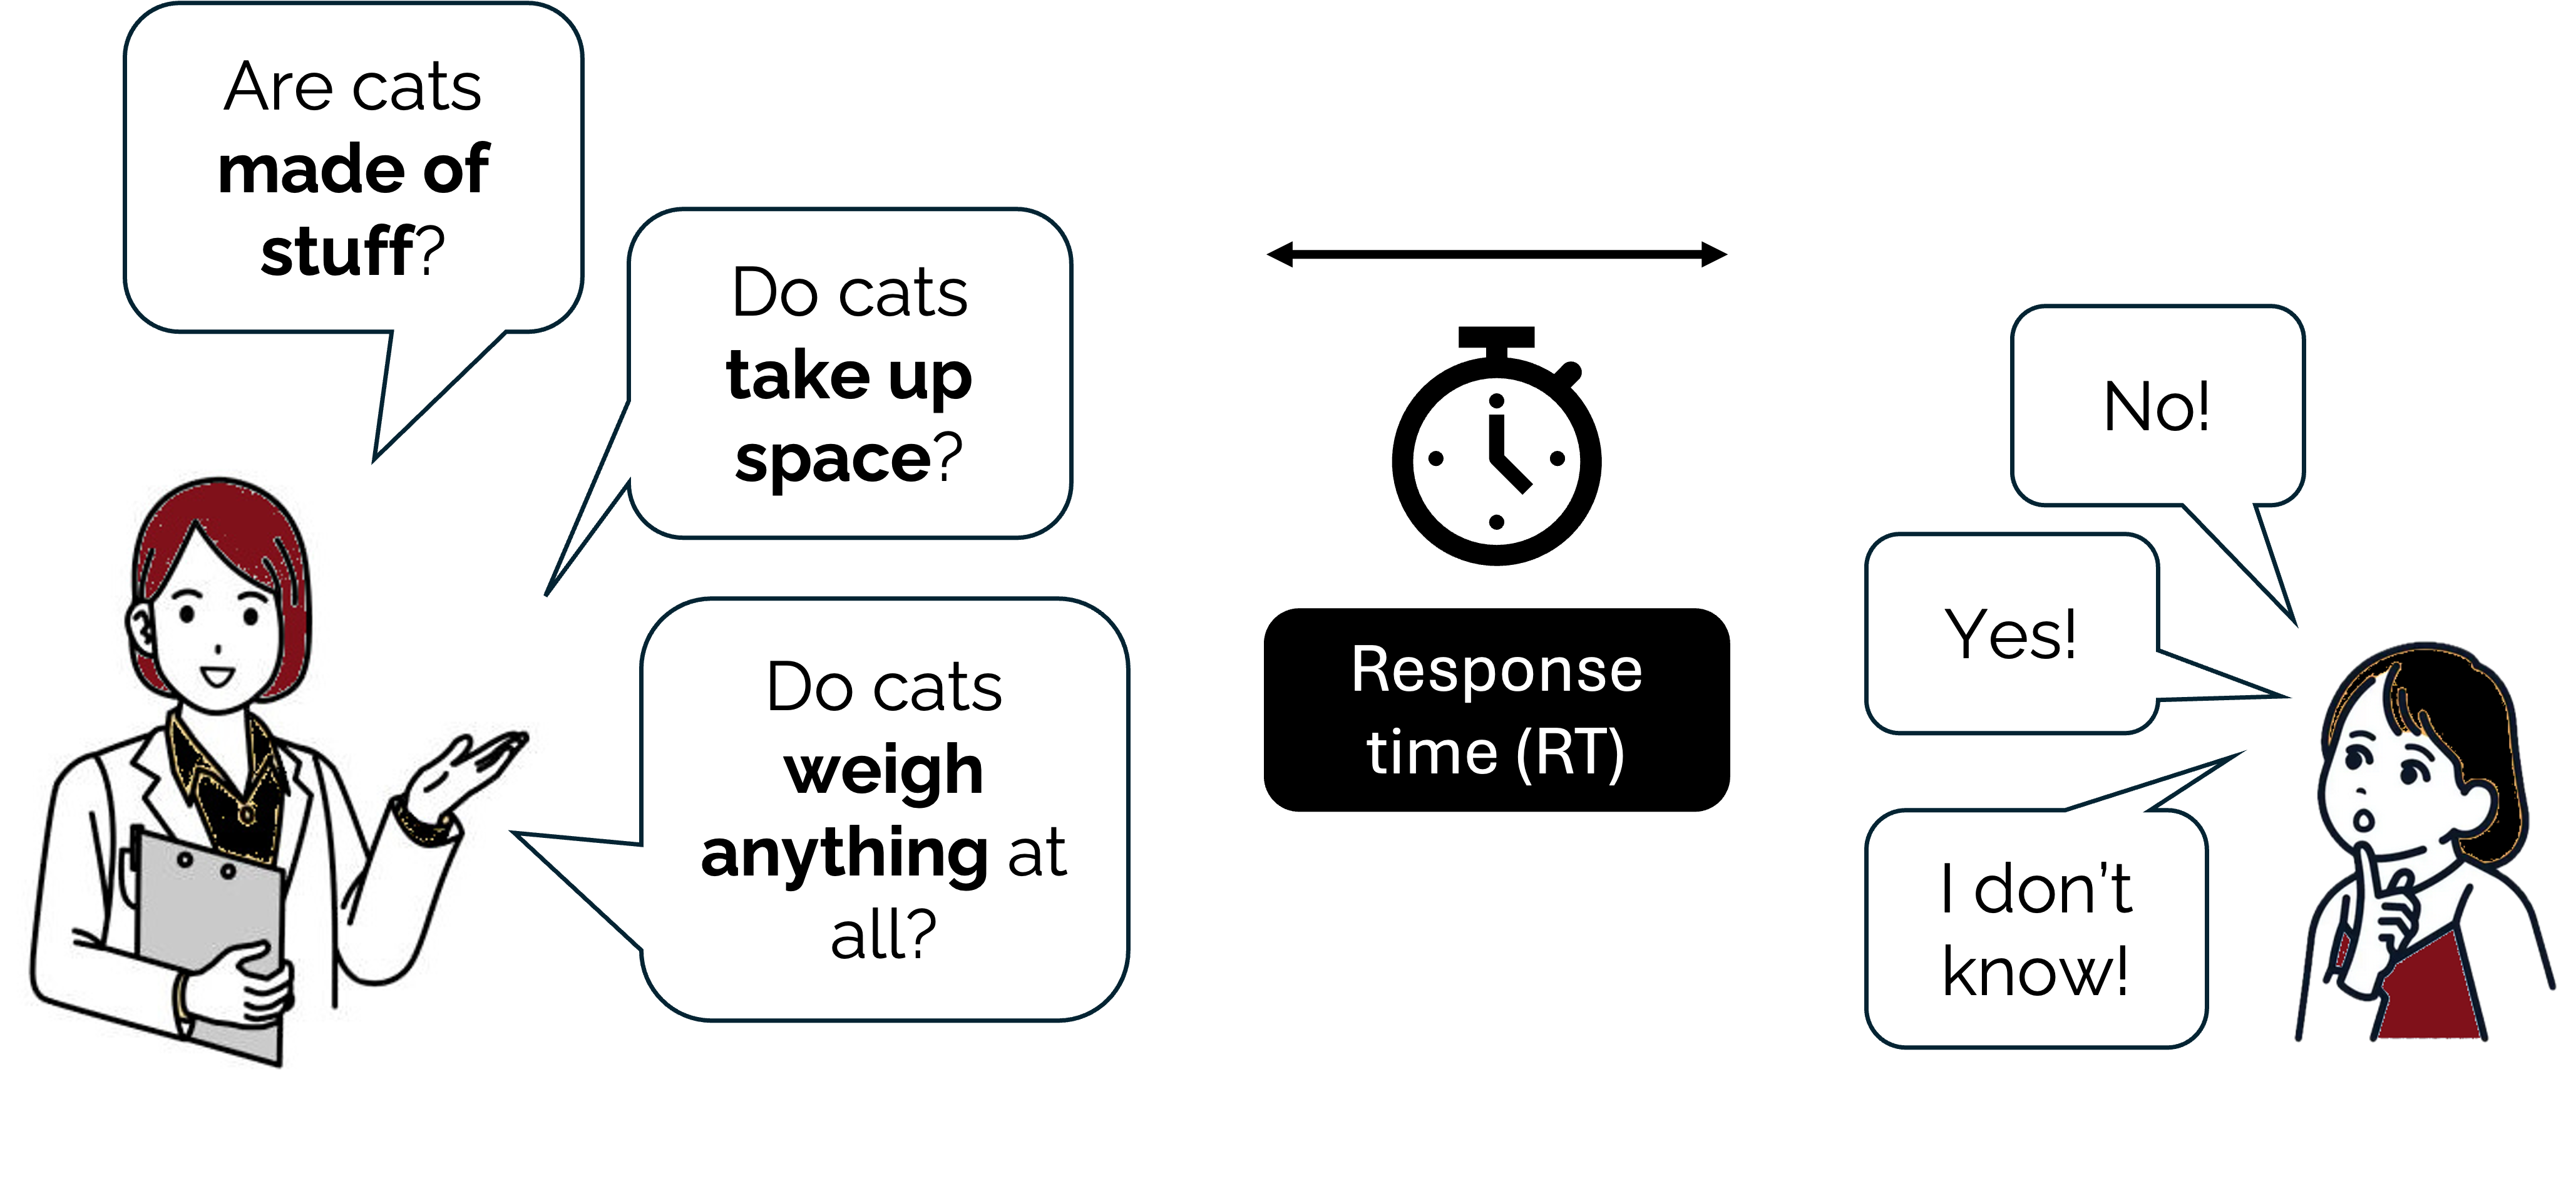
\includegraphics[height=15cm]{images/procedure5.png}}
    \end{figure}

    \begin{itemize}
    	\item \textbf{Congruent questions} (n = 5) were those \textbf{most children} answered \textbf{correctly}; \textbf{incongruent questions} (n = 5) were those \textbf{fewest children} answered \textbf{correctly}
	\item We excluded children's RTs relating to inaccurate and accurate responses, respectively
	\item Based on video, we \textbf{coded children's RTs} (time between end of question and start of response)
    \end{itemize}
    
  \end{block}

\end{column}

\begin{column}{\widecolwidth}

  \begin{block}{RESULTS}

\begin{minipage}{0.55\textwidth}
    \begin{figure}
      \centering
      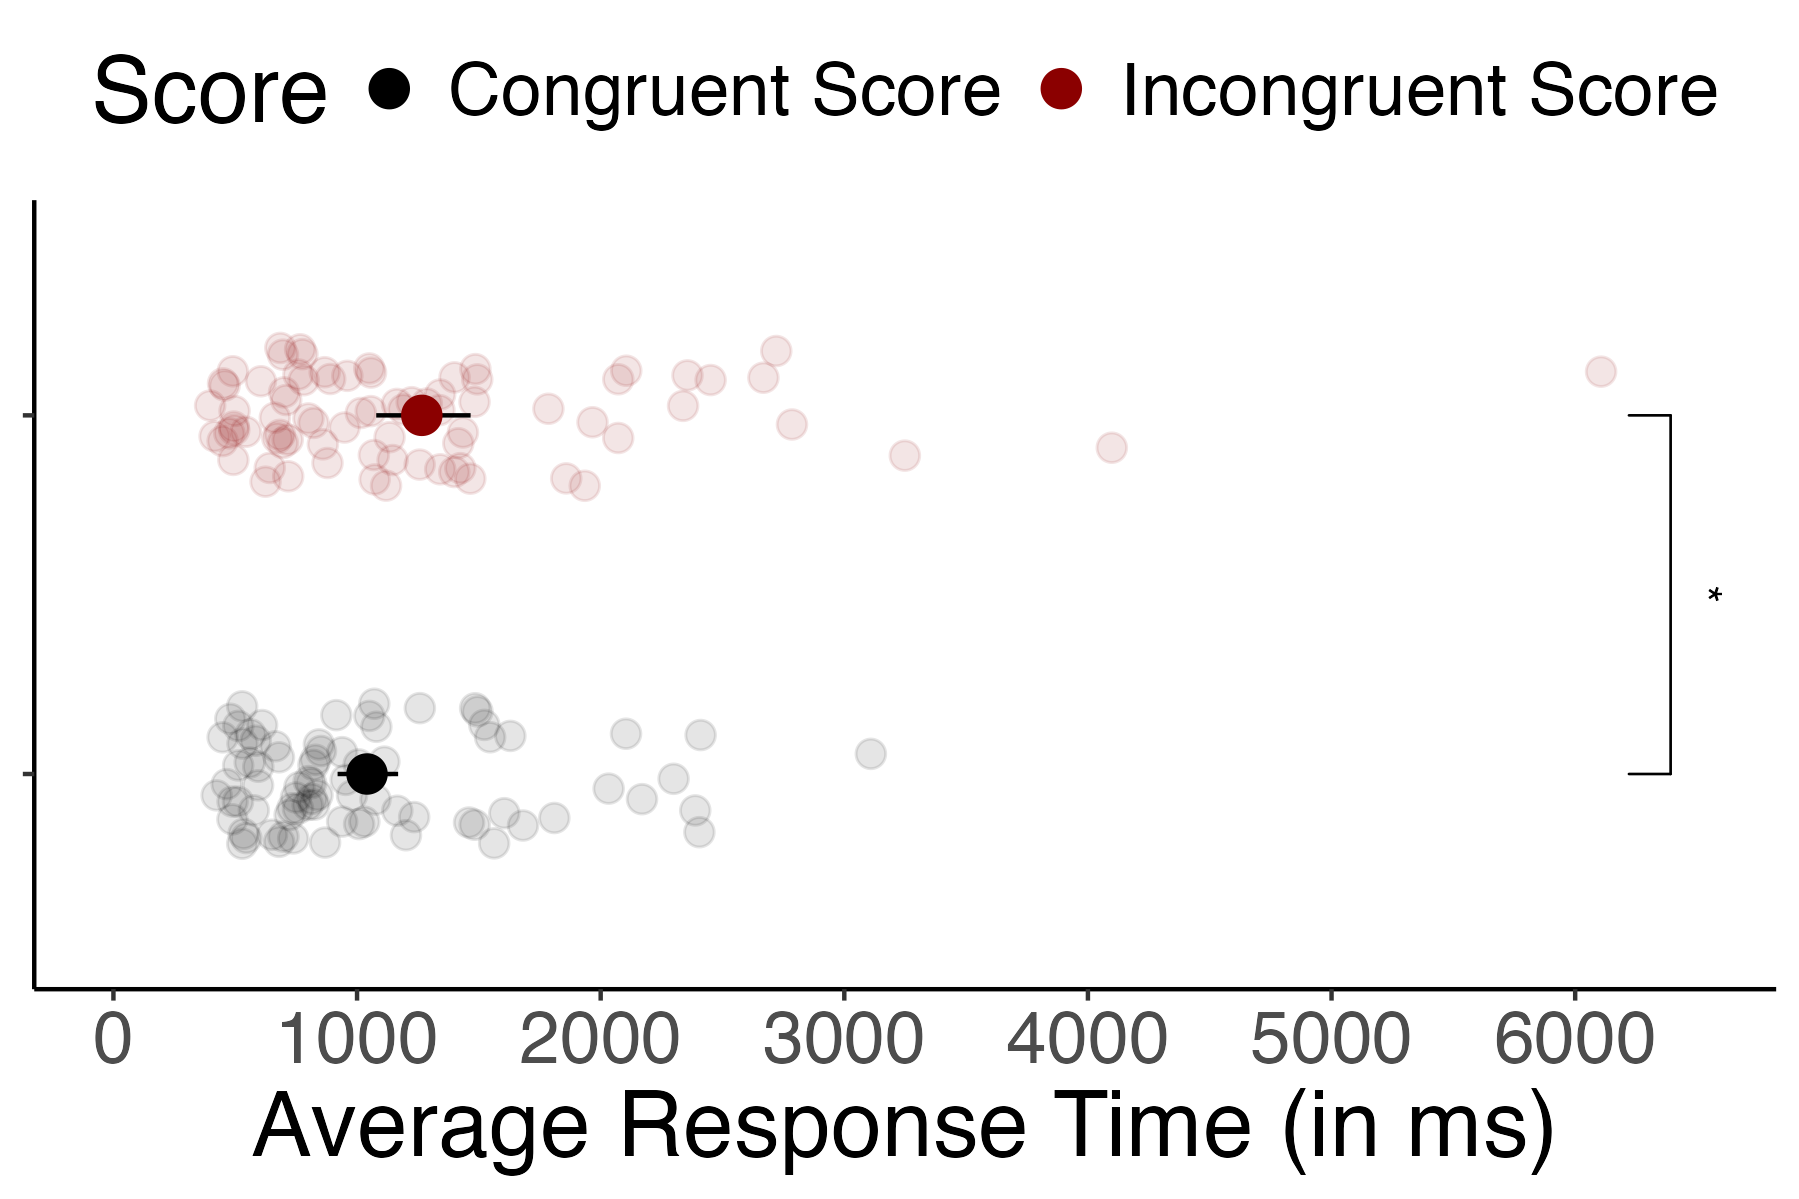
\includegraphics[height=19cm]{plots/figure1.png}
    \end{figure}
\end{minipage}%
\begin{minipage}{0.45\textwidth}
\begin{figure}
      \centering
      \href{https://aspredicted.org/DJG_YWR}{
\includegraphics[height=2.125cm]{images/osf.png}}
      \href{https://aspredicted.org/DJG_YWR}{
\includegraphics[height=2.5cm]{images/aspredicted.png}}
\end{figure}
\center{\Large\textbf{\emph{N} = 79 five- to nine-year-old children} (\emph{M} = X.XX)}\\[2ex]
Mean diff. = 225 ms, \emph{d}  = 0.24 [CIs -0.06, 0.54], \emph{p} = .041; paired t-test (two-tailed)\\[2ex]
    \begin{itemize}
        \item Second coder blind to hypotheses coded 100\% of data; ICC = .84 (congruent); .95 (incongruent)
        \item Overall, children were \textbf{marginally slower to respond to incongruent questions} than congruent ones
        \item \textbf{RTs correlated with EFs} and \textbf{domain knowledge}\newline(\emph{r} = .28, \emph{p} = .021; \emph{r} = .31, \emph{p} = .005)
        \item Variance in RTs did \emph{not} correlate with children's error monitoring or cognitive reflection abilities
    \end{itemize}
\end{minipage}
\end{block}
    
\begin{block}{DISCUSSION \& FUTURE DIRECTIONS}
	\begin{tcolorbox}[
		colback=mycolor,
		colframe=mycolor,
		coltext=white,
		boxsep=2pt,
		left=2mm,
		right=2mm,
		top=2mm,
		bottom=2mm,
		arc=5mm,
		auto outer arc,
		boxrule=4pt,
		width=\dimexpr\linewidth-2\fboxsep\relax,
		]
		\centering
		\textbf{Children's RTs may be informative of their being at the cusp of overturning their naive beliefs about the material world}
	\end{tcolorbox}
	
    \begin{itemize}
      \item \textbf{Even before acquiring a scientific understanding} of matter and its properties, \textbf{elementary schoolers show signs of hesitancy} when producing responses aligned with incorrect naive beliefs
      \item \textbf{Learners vary in their degree of hesitancy}; individual differences relate to levels of EF and overall domain knowledge
      \item We plan to replicate and extend this finding using a question set a) including items beyond the physical reasoning domain, and b), explicitly controlling for age of acquisition and processing-relevant variables (word frequency and length, no. of syllables)
    \end{itemize}
\end{block}

  \begin{block}{REFERENCES}
  \footnotesize
	[1] Carey, S. (2009). The Origin of Concepts. Oxford University Press.\\[1ex]
	[2] Shtulman, A. (2017). Scienceblind: Why Our Intuitive Theories About the World Are So Often Wrong. Hachette UK.\\[1ex]
  \end{block}

\end{column}
\end{columns}
\end{frame}

\end{document}
